\textrm{Test d'un abstract latex :).}

Suspendisse ultricies condimentum volutpat. Donec id massa vitae diam laoreet
tincidunt ac eu massa. Donec faucibus tellus ut metus eleifend egestas. Cras
auctor, mauris viverra euismod iaculis, justo ligula fermentum enim, et
tristique dolor nunc bibendum quam. Quisque iaculis varius arcu, sed pharetra
augue fringilla at. Ut porta condimentum nisl quis eleifend. Pellentesque
auctor dui felis, id iaculis velit. Aliquam mollis, eros vitae luctus dignissim,
nunc mauris euismod ante, in gravida nulla nisl at turpis. Aliquam lacus nulla,
cursus ultricies condimentum ultrices, fringilla vel justo. In hac habitasse
platea dictumst. Quisque viverra elementum ligula, porta placerat sapien
pharetra interdum. Etiam vel nisl dolor, sed mattis sapien. Donec porta auctor
lacus malesuada convallis. Morbi suscipit, eros vitae dignissim pharetra, dui
sem auctor arcu, ac viverra ligula massa euismod nibh. Cras accumsan aliquet
semper. Nunc congue libero non massa egestas in commodo quam accumsan.

\section{Présentation du modèle de représentation de la conscience}
Le modèle dont on s'est inspiré, présenté sur la figure~\ref{modele_original},
représente une vision du fonctionnement que pourrait avoir une conscience
artificielle. En se servant des travaux comme ceux de Freud et de Laborit, il permet de représenter la plupart des caractéristiques
d’une conscience humaine. 
\begin{figure}[H] 
\centering
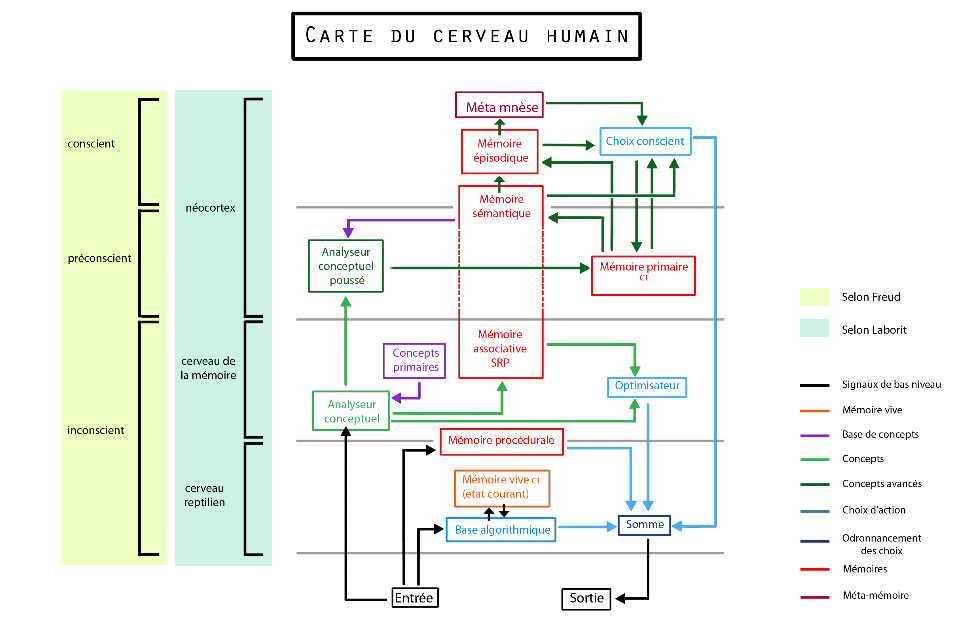
\includegraphics[width=\textwidth]{files/modele_original} 
\caption{Schéma du modèle de représentation de la conscience} 
\label{modele_original}
\end{figure}
